% !TeX root = ../libro.tex
% !TeX encoding = utf8

\chapter{Tratamiento de secuencias}

Hasta ahora se han descrito redes neuronales que tratan los datos de manera aislada. Cada instancia es procesada independientemente y se asigna una salida solo en función de la entrada facilitada. No existe ningún tipo de realimentación en la red. Esta estructura es adecuada para, por ejemplo, problemas de clasificación en los cuales los datos son independientes entre sí y la clasificación de un ejemplo no debería afectar a la del resto. Sin embargo pueden plantearse muchos problemas de aprendizaje en los que no exista tal independencia. El contexto de un ejemplo puede ser relevante para su resolución.

Un caso de este tipo de problemas es el tratamiento de secuencias, conjuntos de datos ordenados en los cuales cada instancia tiene cierta relación con sus antecesores y predecesores. Algunos tipos de datos que podemos interpretar como secuencias son textos, vídeos, grabaciones de voz, cadenas de ADN o música. En las tareas que impliquen su manejo será relevante tener en cuenta la relación de cada elemento con los previos y posteriores. Algunos ejemplos de problemas en los que se usan son:

\begin{itemize}
  \item Generación de texto~\cite{lu2018neural}: consiste en producir texto en lenguaje natural. Puede aplicarse a multitud de fines, entre los que se incluyen completar textos automáticamente, generación de poemas o descripción textual de vídeo o imágenes.
  \item Traducción automática~\cite{singh2017machine}: conversión automática de un lenguaje natural a otro lenguaje natural diferente.
  \item Análisis de secuencias de ADN~\cite{liu2019detection}: dada una secuencia de ADN, detección de determinadas estructuras o modificaciones en el mismo.
  \item Reconocimiento de voz~\cite{graves2013speech}: transcripción del lenguaje hablado captado como audio a texto.
  \item Análisis de sentimientos~\cite{valdivia2017sentiment}: identificación y clasificación de opiniones expresadas en forma de texto para determinar si la actitud de su autor hacia un tema concreto es positiva, negativa o neutral.
  \item Generación de música: creación automática de música. Algunas de las aproximaciones existentes son completar una obra parcialmente compuesta con acompañamientos y contrapunto ~\cite{huang2017counterpoint} o generar música con un estilo determinado ~\cite{carr2018generating}.
\end{itemize}

Además de la dependencia entre elementos es también destacable que por su naturaleza secuencial, los datos con los que trabaja este tipo de problemas pueden ser más extensos de lo que sería práctico computar mediante una red prealimentada profunda. Además pueden tener extensiones diferentes, lo que también resulta problemático. Es por ello que su tratamiento mediante las técnicas vistas hasta ahora resulta muy difícil y se hace necesaria la utilización de modelos especializados.

La principal idea a la hora de enfrentar tareas de esta índole es añadir retroalimentación a la red. De esta manera puede conservarse información a través de las diferentes resoluciones de ejemplos. Cuando se incluye esta característica estamos ante modelos llamados redes neuronales recurrentes (RNN), \textit{recurrent neural networks} en inglés. En este capítulo se repasan las arquitecturas más importantes de este tipo y cómo se afronta el problema de la dependencia entre instancias y la conservación de información entre las sucesivas resoluciones.

\section{Redes neuronales recurrentes}

En este apartado consideramos una secuencia como un conjunto finito de ejemplos $\{\textbf{x}^{(1)},\textbf{x}^{(2)},...,\textbf{x}^{(T)}\}$. Diremos que la secuencia tiene longitud $T$. La idea de introducir retroalimentación en la red es equivalente a introducir un nuevo parámetro a la función que representa la red, al cual llamaremos estado o estado oculto. En cada posición o instante $t$ el estado $\textbf{h}^{(t)}$ dependerá del estado anterior $\textbf{h}^{(t-1)}$ y de la entrada actual $\textbf{x}^{(t)}$. De igual manera, la salida del instante $t$, $\textbf{y}^{(t)}$ ya no solo dependerá de la entrada $\textbf{x}^{(t)}$ y los parámetros $\theta$, sino también del estado anterior $\textbf{h}^{(t-1)}$.

\begin{figure}[htpb]
  \centering
  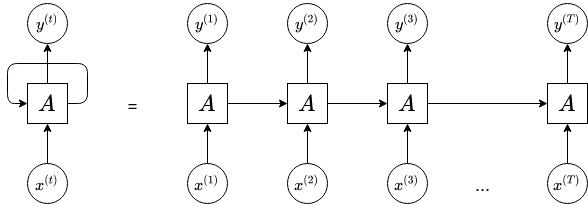
\includegraphics[width=1\textwidth]{recurrent}
  \caption{Desenrollado de una red neuronal recurrente}
  \label{fig:recurrent}
\end{figure}

Para realizar la propagación hacia adelante en una red recurrente como la de la figura (insertar cita a figura anterior) basta con aplicar las siguientes ecuaciones en cada paso $t$, desde $t=1$ hasta $t=T$:
$$\textbf{h}^{(t)} = g_1(\textbf{b} + \textbf{W}\textbf{h}^{(t-1)} + \textbf{U}\textbf{x}^{(t)}), $$
$$\textbf{y}^{(t)} = g_2(\textbf{c} + \textbf{V}\textbf{h}^{(t)}) $$

donde los parámetros son los vectores de de sesgos $\textbf{b}$ y $\textbf{c}$ junto con las matrices de pesos $\textbf{U}$, $\textbf{V}$ y $\textbf{W}$, que conectan la entrada con el estado oculto, el estado oculto con la salida y el estado oculto actual con el siguiente, respectivamente. Las funciones $g_1$ y $g_2$ son funciones de activación que pueden ser diferentes, siendo la primera normalmente una función ReLU o tangente hiperbólica y encargada de generar el siguiente estado y la segunda la encargada de la salida de la red, lo cuál condicionará su forma. Es importante tener en cuenta que todas estas componentes son compartidas por todos los pasos. Por ello esta estructura es equivalente a introducir retroalimentación en la red. Se puede añadir también un estado oculto inicial $\textbf{h}^{(0)}$, cuyo valor será nulo si no tenemos información previa.

La función coste total para una secuencia se calcula como la suma de los costes para cada uno de sus pasos. Calcular el gradiente de esta con respecto de cada parámetro es una operación computacionalmente costosa, ya que implica realizar una propagación hacia adelante de izquierda a derecha del modelo a través de cada uno de los pasos y después una propagación hacia atrás en sentido contrario a través de todo el grafo. El tiempo de ejecución es $O(T)$ y no puede ser reducido mediante paralelización ya que los grafos con los que trabajamos son secuenciales por definición. Los estados calculados en la propagación hacia adelante deben ser almacenados hasta su utilización en la propagación hacia atrás, por lo que el coste de memoria también es $O(T)$. Las redes recurrentes son por tanto muy útiles en muchos casos, pero también muy costosas de entrenar.

\subsection{Arquitecturas más comunes}

Hasta ahora se ha supuesto que la entrada y la salida tienen la misma longitud, pero no tiene por qué ser así. De hecho, uno de los problemas que solucionaba el uso de redes neuronales recursivas era la desigualdad en dichas longitudes. Veamos las diferentes situaciones que pueden darse en este sentido y los modelos resultantes.

\begin{itemize}
\item Arquitectura \textit{one-to-one}: las redes tradicionales son un caso particular de las redes recurrentes en el que tanto la entrada como la salida tienen una longitud $T_x = T_y = 1$.
\item Arquitectura \textit{one-to-many}: en este caso la longitud de la entrada es uno, $T_x = 1$, pero la de la salida es mayor que uno, $T_y > 1$. En este caso, para $t \in \{2,...,T\}$ se añade como entrada la salida del instante anterior, $\textbf{y}^{(t-1)}$. Esta arquitectura suele aplicarse en generación de texto o música.
\item Arquitectura \textit{many-to-one}: al contrario que en el caso anterior, ahora $T_x > 1$ y $T_y = 1$. Con estas condiciones solo el último instante de la red tendrá salida, mientras que el resto solo leerán la secuencia de entrada y generan los respectivos estados ocultos. Es útil, por ejemplo, para clasificar o etiquetar secuencias. Una aplicación es el ya visto análisis de sentimientos.
\item Arquitectura \textit{many-to-many}, igual longitud: en este caso la secuencia de entrada y de salida tienen la misma longitud. Es la representada al principio del apartado. Se utiliza en casos en los que la secuencia de entrada y de salida están directamente relacionadas, como por ejemplo para el reconocimiento de entidades en un texto.
\item Arquitectura codificador-decodificador: se trata de otra variante de la arquitectura \textit{many-to-many}, pero en este caso $T_x \neq T_y$. Podemos verla como la unión de dos estructuras. La primera, el codificador, lee la secuencia de entrada sin producir salida una salida y genera los estados ocultos correspondientes. La segunda, el decodificador, produce las salidas sin una entrada, solo a través de los estados ocultos. Tiene múltiples utilidades como la traducción automática o el reconocimiento de voz.

\end{itemize}

\begin{figure}[htpb]
  \centering
  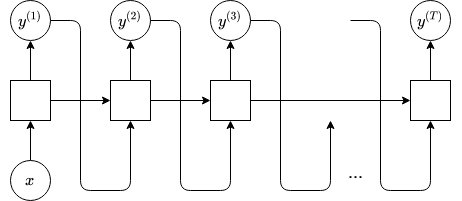
\includegraphics[width=0.8\textwidth]{onetomany}
  \caption{Red recurrente con arquitectura \textit{one-to-many}}
  \label{fig:onetomany}
\end{figure}

\begin{figure}[htpb]
\centering
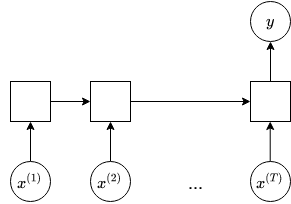
\includegraphics[width=0.6\textwidth]{manytoone}
\caption{Red recurrente con arquitectura \textit{many-to-one}}
\label{fig:manytoone}
\end{figure}

\begin{figure}[htpb]
  \centering
  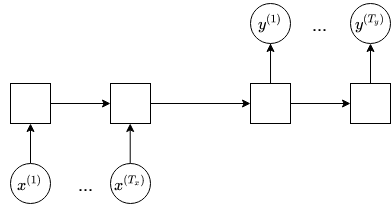
\includegraphics[width=0.75\textwidth]{encoderdecoder}
  \caption{Red recurrente con arquitectura codificador-decodificador}
  \label{fig:encoderdecoder}
\end{figure}


\subsection{Redes recurrentes bidireccionales}\label{rnn-bidirec}

Las redes recursivas mencionadas hasta el momento, en el instante $t$, solo capturan información de las entradas pasadas y presentes, $\textbf{x}^{(1)},...,\textbf{x}^{(t-1)},\textbf{x}^{(t)}$. En muchas aplicaciones, sin embargo, la salida deseada no depende solo de las posiciones previas en la secuencia, sino de la secuencia de entrada completa. Podemos encontrar un ejemplo de esto en el reconocimiento de voz. La correcta interpretación de un fonema puede depender de los siguientes, o incluso de las siguientes palabras. Si hay varias interpretaciones de una palabra, ambas acústicamente plausibles, puede ser necesario recurrir a la información que se tiene del futuro y del pasado para elegir la más correcta. Las redes neuronales recurrentes bidireccionales (RNNs bidireccionales) se crearon para afrontar este tipo de problemas.

Las redes recurrentes bidireccionales combinan dos redes recurrentes, una que avanza hacia adelante en el tiempo, desde el principio hasta al final de la secuencia de entrada, y otra que se mueve en dirección contraria, desde el final de la secuencia de entrada hasta su principio. La salida de cada instante dependerá de los estados ocultos de ambas subredes. De esta manera las unidades de salida producen una representación que depende del pasado y del futuro, y que es más sensible a entradas cercanas en el tiempo.

\begin{figure}[htpb]
  \centering
  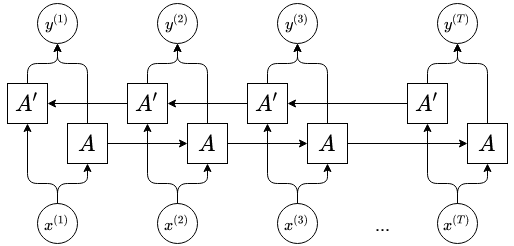
\includegraphics[width=1\textwidth]{bidirectional}
  \caption{Red recurrente bidireccional}
  \label{fig:bidirectional}
\end{figure}

\subsection{Redes recurrentes profundas}\label{rnn-deep}

Podemos clasificar las operaciones que realizan la mayoría de redes neuronales profundas en tres categorías de parámetros y sus transformaciones asociadas:

\begin{enumerate}
\item desde la entrada hasta el estado oculto,
\item desde el estado oculto previo hasta el siguiente estado oculto y
\item desde el estado oculto a la salida.
\end{enumerate}

Hasta ahora cada uno de estos bloques ha estado asociado a una única matriz de pesos, es decir, realiza una transformación que puede ser representada por una única capa de una red prealimentada profunda. La evidencia experimental (\cite{graves2013speech}, \cite{pascanu2013construct}) sugiere que puede ser beneficioso introducir una mayor profundidad en cada una de las categorías. Si se piensa en la capacidad de representación, aumentar la profundidad resulta beneficioso. Sin embargo puede ser contraproducente para el aprendizaje, ya que hace la optimización más difícil.

La profundidad de una red recurrente puede aumentarse añadiendo capas ocultas, que pueden introducirse como capas ocultas recurrentes o como capas previas o posteriores a la capa o capas recurrentes. La estructura de una red recurrente profunda queda reflejada en la \autoref{fig:deeprecurrent}.

\begin{figure}[htpb]
  \centering
  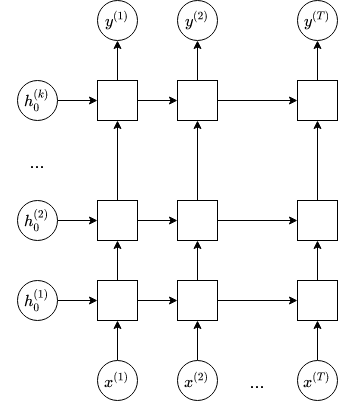
\includegraphics[width=0.6\textwidth]{deeprecurrent}
  \caption{Red recurrente profunda}
  \label{fig:deeprecurrent}
\end{figure}

\section{Dependencia a largo plazo}

Para muchas de las aplicaciones que hemos visto hasta ahora de las redes neuronales recurrentes es importante que el modelo conserve cierta información a través del tiempo hasta instantes lejanos. Cuando los grafos de los modelos usados se vuelven muy profundos, y especialmente en el caso de las redes recurrentes en las que la profundidad consiste en la aplicación múltiples veces de la misma operación, surgen problemas en el aprendizaje. En esta sección se describe el motivo de estos problemas y algunas propuestas para su afrontamiento.

\subsection{Problemas del gradiente en redes recurrentes}

El problema clave en el aprendizaje de dependencias a largo plazo es que el gradiente, propagado a través de gran cantidad de etapas, tiende a desvanecerse hacia valores casi nulos en la mayoría de los casos o, más raramente pero siendo más dañino para la optimización, a explotar hacia valores muy grandes. Estos son los conocidos como \textit{vanishing gradient problem} y \textit{exploding gradient problem}.

Las redes recurrentes se basan en la composición de la misma función, una vez cada paso. La composición sucesiva de funciones no lineales puede resultar en un comportamiento extremadamente no lineal, con una gran mayoría de valores con derivada casi nula, algunos valores con derivadas muy grandes y gran cantidad de alteraciones entre crecimiento y decrecimiento.

En particular, la composición empleada por las redes recurrentes neuronales es parecida a la multiplicación de matrices. Podemos tomar un ejemplo simplificado con $$\textbf{h}^{(t)} = \textbf{W}^T\textbf{h}^{(t-1)},$$ una red recurrente muy simple con función de activación lineal y sin entrada. En este caso, la aplicación del paso $t$-ésimo consiste en multiplicar la matriz de pesos \textbf{W} traspuesta con el estado anterior. Por lo tanto llegar al estado $t$-ésimo es, simplemente, aplicar esta operación $t$ veces sobre el estado inicial, $$\textbf{h}^{(t)} = \left( \textbf{W}^t \right)^T \textbf{h}^{(0)}.$$ Suponiendo $\textbf{W}$ diagonalizable, con $$ \textbf{W} = \textbf{Q}\textbf{A}\textbf{Q}^T, $$ con $\textbf{Q}$ ortogonal, podemos expresar $$\textbf{h}^{(t)} = \textbf{Q}^T\textbf{A}^t\textbf{Q}\textbf{h}^{(0)}. $$

Los valores propios están elevados a $t$, lo que produce que aquellos con valor propio menor que $1$ tenderán a desvanecerse hacia 0 y los que tengan valor propio mayor que $1$ a explotar con valores muy grandes. Por tanto, cualquier componente de $\textbf{h}^{(0)}$ que no esté alineada con valores propios grandes será descartada.

A continuación se exponen algunas alternativas a las redes recurrentes cuyo objetivo es evitar problemas con el gradiente y memorizar así dependencias a largo plazo.

\subsection{Redes recurrentes con puertas}

Los modelos que han demostrado ser más efectivos en aplicaciones prácticas para el uso de secuencia son las redes neuronales recursivas con puertas (\textit{gated RNNs}). Estos se basan en la idea de crear caminos a lo largo del tiempo cuyo gradiente no se desvanezca ni explote. A través de estos las redes recursivas con puertas podrán acumular información. Cuándo la información se almacena y se descarta será también aprendido por la red. Existen dos alternativas principales, modelos con memoria larga a corto plazo (\textit{long-short term memory, LSTM}), y las redes basadas en unidades recurrentes con puertas (\textit{gated recurrent unit, GRU}).

\subsubsection{LSTM}\label{lstm}

Las unidades de las redes neuronales simples son sustituidas por estructuras más complejas, a las que se llama bloques LSTM. Así, una red con LSTM tiene la misma forma de cadena de una RNN, pero utilizando estas nuevas estructuras cuyo comportamiento está dirigido a conservar información en el largo plazo~\cite{hochreiter1997long}.

\begin{figure}[htpb]
  \centering
  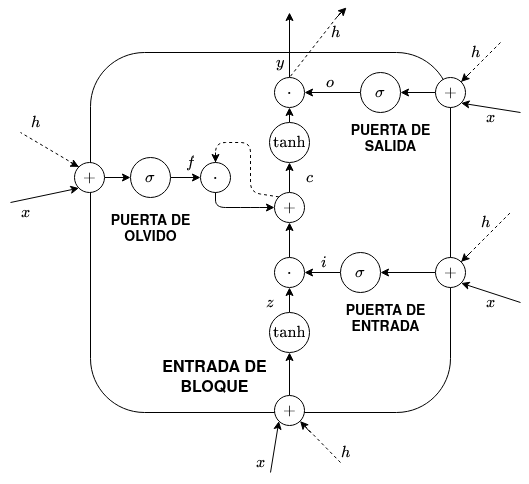
\includegraphics[width=1\textwidth]{LSTM}
  \caption{Bloque LSTM. Las líneas discontinuas representan conexiones con retardo en el tiempo}
  \label{fig:LSTM}
\end{figure}

La estructura de una célula es la representada en la gráfica \autoref{fig:LSTM}. La adición clave es una celda de memoria en cada bloque, $\textbf{c}^{(t)}$. La información que se se almacena desde la entrada y el estado oculto en la celda y que se entrae de la misma hacia la salida viene filtrada por diferentes puertas, unidades con su correspondiente función de activación.

El primer paso es decidir qué información se elimina de la celda. Esta decisión se realiza mediante la puerta de olvido, que contiene una unidad sigmoidal cuyas entradas son el estado oculto anterior $ \textbf{h}^{(t-1)}$ y la entrada del bloque $\textbf{x}^{(t)}$. Su salida $\textbf{f}^{(t)}$, entre $0$ y $1$, señala con qué intensidad se mantiene la información de la celda.

El siguiente paso es decidir qué nueva información se almacena en la celda. Se realiza en dos etapas. En la primera una unidad sigmoidal llamada puerta de entrada decide qué valores se actualizarán. Después una unidad $\tanh$ crea un vector con los nuevos datos candidatos $\textbf{z}^{(t)}$, que serán sumados a la celda. Por último se combinan estos dos pasos, multiplicando coordenada a coordenada, para definir finalmente la actualización de la celda.

A continuación se actualiza el estado anterior de la celda. Basta multiplicar coordenada a coordenada el estado anterior por el vector obtenido en la puerta de olvido y sumarle el vector obtenido en la puerta de entrada.

Por último se procesa la salida, que será una versión filtrada de la celda de memoria utilizando la entrada y el estado oculto anterior. El estado oculto y la entrada son transformadas por una unidad sigmoidal. El estado actual de la célula pasa por una unidad de $\tanh$ y se multiplica componente a componente su salida con la de la puerta de salida.

Podemos resumir el modelo en las siguientes ecuaciones, donde $\odot$ representa el producto componente a componente~\cite{greff2016lstm}:

\begin{itemize}
\item Entrada de bloque: $\textbf{z}^{(t)} = \tanh(\textbf{W}_z \textbf{x}^{(t)} +  \textbf{R}_z \textbf{h}^{(t-1)}  + \textbf{b}_z)$
\item Puerta de entrada: $\textbf{i}^{(t)} = \sigma(\textbf{W}_i\textbf{x}^{(t)} + \textbf{R}_i \textbf{h}^{(t-1)} + \textbf{b}_i)$
\item Puerta de olvido: $\textbf{f}^{(t)} = \sigma(\textbf{W}_f \textbf{x}^{(t)} + \textbf{R}_f\textbf{h}^{(t-1)} + \textbf{b}_f)$
\item Celda: $\textbf{c}^{(t)} = \textbf{z}^{(t)}\odot \textbf{i}^{(t)} + \textbf{c}^{(t-1)} \odot \textbf{f}^{(t)}$
\item Puerta de salida: $\textbf{o}^{(t)} = \sigma(\textbf{W}_o \textbf{x}^{(t)} + \textbf{R}_o \textbf{h}^{(t-1)} + \textbf{b}_o)$
\item Salida de bloque: $\textbf{h}^{(t)} = \tanh (\textbf{c}^t) \odot \textbf{o}^{(t)}$
\end{itemize}

donde $\textbf{W}_z$, $\textbf{W}_i$, $\textbf{W}_f$, $\textbf{W}_o$ son las matrices de pesos para la entrada en cada una de las unidades, $\textbf{R}_z$, $\textbf{R}_i$, $\textbf{R}_f$, $\textbf{R}_o$ las matrices de pesos para los estados ocultos previos y $\textbf{b}_z$, $\textbf{b}_i$, $\textbf{b}_f$, $\textbf{b}_o$ los respectivos vectores de sesgos.

Sobre el bloque LSTM visto hasta ahora pueden introducirse varias modificaciones. La más popular es la que introduce conexiones de mirilla (\textit{peephole connections})~\cite{gers2000recurrent}, mediante las cuales se conecta el estado de la celda de memoria con cada una de las unidades de las puertas. Estas conexiones pueden añadirse a todas las puertas o solo a algunas.

\begin{figure}[htpb]
  \centering
  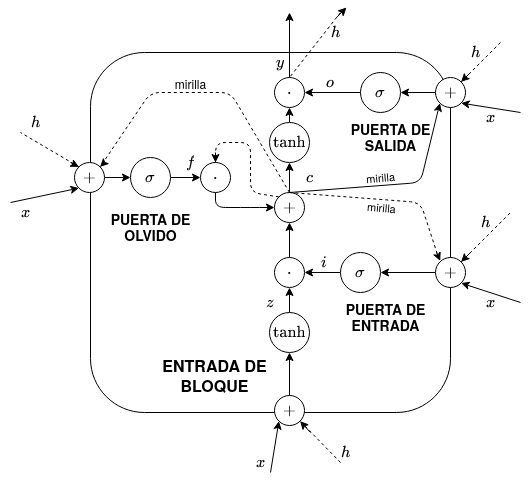
\includegraphics[width=1\textwidth]{LSTM-peephole}
  \caption{Bloque LSTM con conexiones de mirilla. Las líneas discontinuas representan conexiones con retardo en el tiempo}
  \label{fig:LSTM-peephole}
\end{figure}

\subsubsection{GRU}

Una variación que surge de la simplificación de las celdas LSTM vistas anteriormente son las unidades recurrentes con puertas (\textit{gated  recurrent unit}, GRU)~\cite{cho2014learning}. La principal diferencia es que combina la puerta de entrada y la puerta de olvido en una sola unidad, la puerta de actualización (\textit{update gate}). Tampoco diferencia entre estado oculto y celda de memoria, por lo que no es necesario el uso de una puerta de salida. A continuación se describe su funcionamiento detalladamente.

\begin{figure}[htpb]
  \centering
  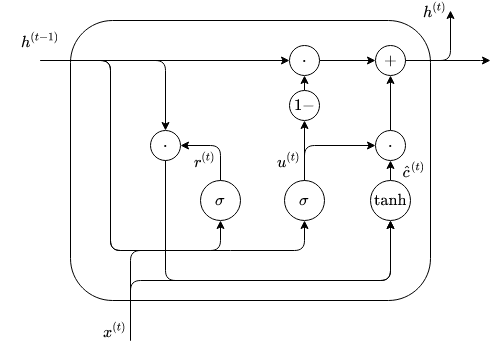
\includegraphics[width=0.9\textwidth]{gru}
  \caption{Bloque GRU}
  \label{fig:gru}
\end{figure}


Primeramente el estado previo anterior $\textbf{h}^{(t-1)}$ y la entrada actual $\textbf{x}^{(t)}$ son filtrados a través de la puerta de relevancia, que normalmente es una unidad sigmoidal. Su salida $\textbf{r}^{(t)}$ indica cómo de relevante es el estado oculto previo.

A continuación se calcula el valor $\textbf{u}^{(t)}$ de la puerta de actualización mediante otra unidad sigmoidal. El valor $1 - \textbf{u}^{(t)}$ sustituye al que en LSTM correspondería a la salida de la puerta de olvido.

Los datos candidatos se calculan, por tanto, aplicando una unidad $\tanh$ a la multiplicación componente a componente de la salida de la puerta de relevancia, $\textbf{r}^{(t)}$, y la entrada actual, $\textbf{x}^{(t)}$. La actualización del estado oculto se realiza entonces sumando la multiplicación componente a componente de los datos candidatos por la salida de la puerta de actualización con el producto componente a componente de $1 - \textbf{u}^{(t)}$ con el valor oculto anterior.

Podemos resumir el modelo en las siguientes ecuaciones, donde $\odot$ representa el producto componente a componente:

\begin{itemize}
\item Puerta de relevancia: $ \textbf{r}^{(t)} = \sigma(\textbf{W}_r\textbf{x}^{(t)} + \textbf{R}_r \textbf{h}^{(t-1)} + \textbf{b}_r)$
\item Puerta de actualización: $ \textbf{u}^{(t)} = \sigma(\textbf{W}_u\textbf{x}^{(t)} + \textbf{R}_u \textbf{h}^{(t-1)} + \textbf{b}_u)$
\item Candidato a estado oculto: $\hat{\textbf{c}}^{(t)} = \tanh(\textbf{W}_c\textbf{x}^{(t)} + \textbf{R}_c( \textbf{r}^{(t)} \odot \textbf{h}^{(t-1)}) + \textbf{b}_c)$
\item Salida: $\textbf{h}^{(t)} = (1- \textbf{u}^{(t)}) \odot \textbf{h}^{(t-1)} + \textbf{z}^{(t)} \odot \hat{\textbf{c}}^{(t)}$
\end{itemize}

donde $\textbf{W}_r$, $\textbf{W}_u$, $\textbf{W}_c$ son las matrices de pesos para la entrada en cada una de las unidades, $\textbf{R}_r$, $\textbf{R}_u$, $\textbf{R}_c,$ las matrices de pesos para los estados ocultos previos y $\textbf{b}_r$, $\textbf{b}_u$, $\textbf{b}_c$ los respectivos vectores de sesgos.


\endinput
%------------------------------------------------------------------------------------
% FIN DEL CAPÍTULO.
%------------------------------------------------------------------------------------
